% adc-ntc.tex
% 

\documentclass[11pt,a4paper]{article}

\usepackage{graphicx}
\usepackage{indentfirst}
\usepackage{verbatim}
\usepackage{amsmath}
%\usepackage{textcomp}
%\usepackage{multirow}
%\usepackage{fancybox}
%\usepackage{endnotes}

\title{NTC Thermometer: ADC of ATmega48}
\author{sun\_ge@yahoo.cn}

\begin{document}

\maketitle


\section{Project Origin}
In order to get current temperature, the cheapest way is using a ATmega48, which has 10-bits ADC unit,
and a NTC (Negative Temperature Coefficient) resistor. It's as accurate as a temperature sensor like
LM35, with lower cost.\\

\begin{center}
The following picture shows the temperature measured by LM35 ($23.8^\circ C$) and 
temperature measured by NTC ($23.4^\circ C$) at same time. 
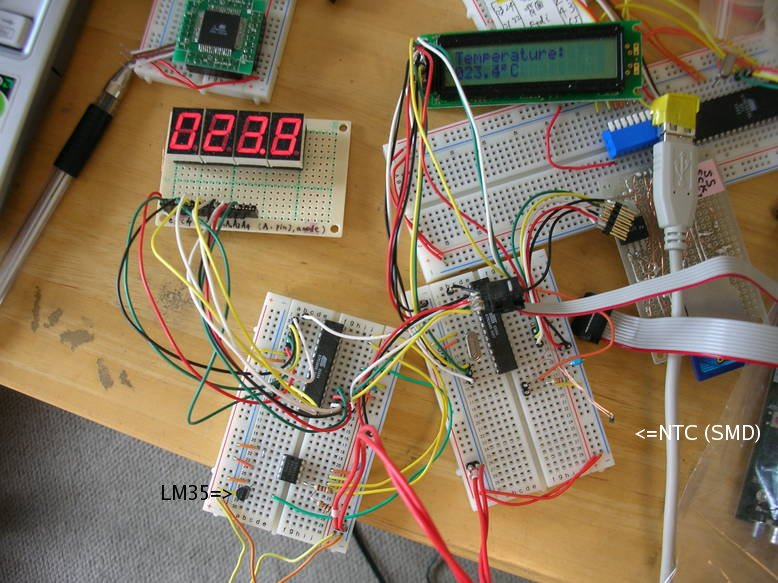
\includegraphics[scale=0.8]{adc-cmp.jpg}
\end{center}

\section{Hardware}
\verbatiminput{hardware.txt}

\section{Source Code}
Source contains: lcd.h, lcd.c, ntc-adc.c and Makefile.\\
It can be compiled and installed by AVR GNU Tools Chain.

\subsection{LCD Library Header: lcd.h}
\verbatiminput{lcd.h}

\subsection{LCD Library: lcd.c}
\verbatiminput{lcd.c}

\subsection{Main Program: ntc-adc.c}
\verbatiminput{ntc-adc.c}

\subsection{Makefile}
\verbatiminput{Makefile}

\end{document}

%%% Local Variables:
%%% coding: UTF-8
%%% mode: latex
%%% End:
